% Created 2025-03-26 Wed 14:53
% Intended LaTeX compiler: pdflatex
\documentclass[bigger]{beamer}
\usepackage[utf8]{inputenc}
\usepackage[T1]{fontenc}
\usepackage{graphicx}
\usepackage{grffile}
\usepackage{longtable}
\usepackage{wrapfig}
\usepackage{rotating}
\usepackage[normalem]{ulem}
\usepackage{amsmath}
\usepackage{textcomp}
\usepackage{amssymb}
\usepackage{capt-of}
\usepackage{hyperref}
\usepackage[spanish, mexico, english]{babel}
\uselanguage{Spanish}
\languagepath{Spanish}
\usepackage{mathtools}
%%%%%%%%%%%%%%%%%%%%%%%%%%%%%%%%%%%%%%%%%%%%%%%%%%%%%%%%%%%%%%%%%%%%%%%%%%%%%%%%%%%%%%%%
%% TEX code to draw an external link symbol                                           %%
%% See https://tex.stackexchange.com/questions/99316/symbol-for-external-links/294990 %%
%%%%%%%%%%%%%%%%%%%%%%%%%%%%%%%%%%%%%%%%%%%%%%%%%%%%%%%%%%%%%%%%%%%%%%%%%%%%%%%%%%%%%%%%

\usepackage{tikz}

\newcommand{\ExternalLink}{%
    \tikz[x=1.2ex, y=1.2ex, baseline=-0.05ex]{% 
        \begin{scope}[x=1ex, y=1ex]
            \clip (-0.1,-0.1) 
                --++ (-0, 1.2) 
                --++ (0.6, 0) 
                --++ (0, -0.6) 
                --++ (0.6, 0) 
                --++ (0, -1);
            \path[draw, 
                line width = 0.5, 
                rounded corners=0.5] 
                (0,0) rectangle (1,1);
        \end{scope}
        \path[draw, line width = 0.5] (0.5, 0.5) 
            -- (1, 1);
        \path[draw, line width = 0.5] (0.6, 1) 
            -- (1, 1) -- (1, 0.6);
    }
}


\usepackage{transparent}
\usetheme{Pittsburgh}
\usecolortheme{dove}
\author{Eric Magar}
\date{28-3-2025 \newline Univ. of Houston}
\title{In remembrance of Francisco Cantú}
\setbeamertemplate{footline}[frame number]{}
\setbeamertemplate{navigation symbols}{}
\expandafter\def\expandafter\insertshorttitle\expandafter{%
\insertshorttitle\hfill%
\insertframenumber}
%  \insertframenumber\,/\,\inserttotalframenumber}
\hypersetup{
 pdfauthor={Eric Magar},
 pdftitle={In remembrance of Francisco Cantú},
 pdfkeywords={},
 pdfsubject={},
 pdfcreator={Emacs 27.1 (Org mode 9.3)}, 
 pdflang={English}}
\begin{document}

\maketitle
\begin{frame}{Outline}
\tableofcontents
\end{frame}

\setbeamercovered{transparent}

\section{Pubs}
\label{sec:org4b2603b}
\begin{frame}[label={sec:orgf89d63b}]{Team player}
\begin{columns}
\begin{column}{0.5\columnwidth}
\begin{itemize}
\item Susan Achury
\item Leonardo Antenangeli
\item Natalia Aruguete
\item Ernesto Calvo
\item Scott Clifford
\item Scott Desposato (x2)
\item Cengiz Erisen
\item Jorge Fernandes
\item Omar García Ponce
\item Agustina Haime
\item Victor Hernández Huerta
\item Verónica Hoyo (x2)
\item Paul Johnson
\item Sandra Ley (x2)
\end{itemize}
\end{column}
\begin{column}{0.5\columnwidth}
\begin{itemize}
\item Eric Magar
\item Marco Morales
\item Javier Márquez
\item Margarita Ramírez
\item Pedro Riera (x3)
\item Sebastián Saiegh
\item Carlos Scartascini
\item Leslie Schwindt-Bayer
\item Robert Stein et al. (x2)
\item Michelle Torres
\item Agustín Vallejo
\item Tiago Ventura
\item Dane Wendell
\end{itemize}
\end{column}
\end{columns}
\end{frame}
\begin{frame}[label={sec:orgfc0634f}]{Tres vetas}
\begin{block}{Fraude, integridad electoral}
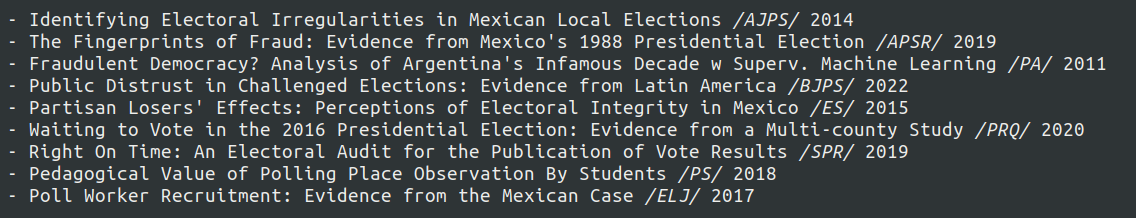
\includegraphics[width=\textwidth]{./pics/pubs1.png}
\end{block}
\begin{block}{Votos, compra-venta}
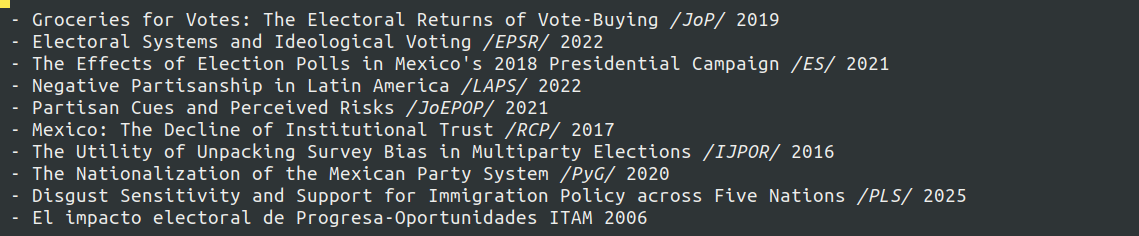
\includegraphics[width=\textwidth]{./pics/pubs2.png}
\end{block}
\begin{block}{Estudios legislativos}
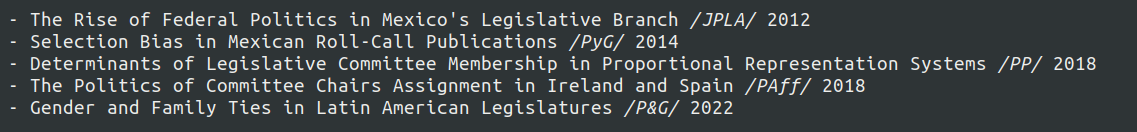
\includegraphics[width=\textwidth]{./pics/pubs3.png}
\end{block}
\end{frame}
\begin{frame}[label={sec:org5ce83c4}]{Tres vetas}
\begin{block}{Fraude, integridad electoral}
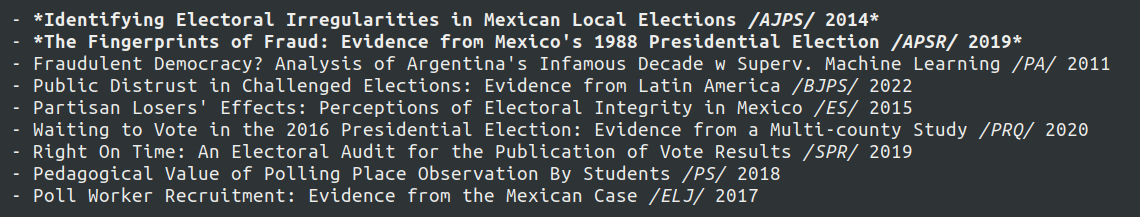
\includegraphics[width=\textwidth]{./pics/pubs1s.png}
\end{block}
\begin{block}{Votos, compra-venta}
\transparent{0.3}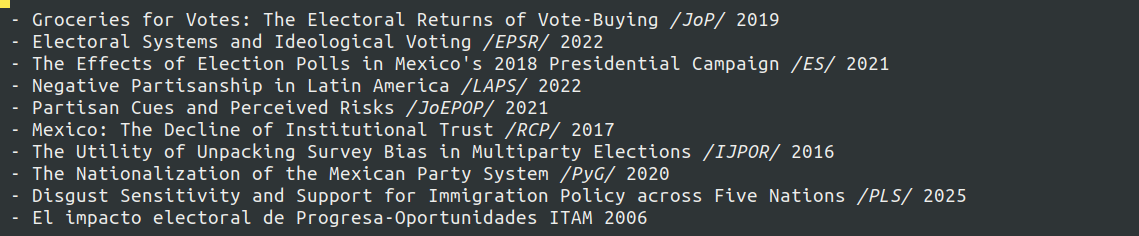
\includegraphics[width=\textwidth]{./pics/pubs2.png}
\end{block}
\begin{block}{Estudios legislativos}
\transparent{0.3}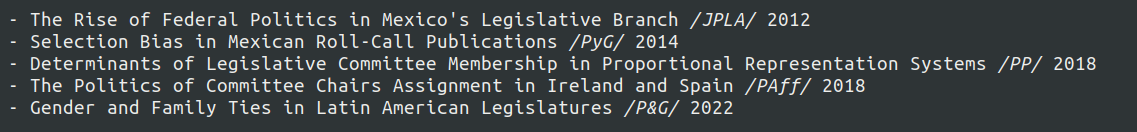
\includegraphics[width=\textwidth]{./pics/pubs3.png}
\end{block}
\end{frame}

\section{Mi presentación}
\label{sec:org61ab052}
\begin{frame}[label={sec:org4449191}]{}
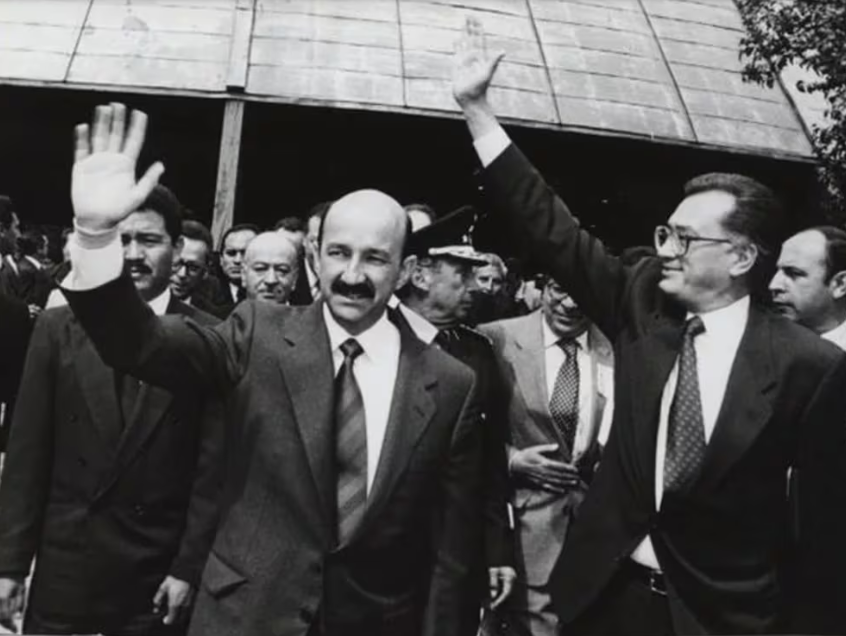
\includegraphics[width=\textwidth]{./pics/csg-bartlett.png}
\end{frame}
\begin{frame}[label={sec:org797d352}]{Aire fresco para una controversia añeja}
\begin{itemize}
\item CFE reportó cómputos agregados de consejos distritales $$V = \sum_{d=1}^{300} v_d = 9.6M~~(50.3\%)$$
\end{itemize}
\pause
\begin{itemize}
\item 30 años sin evidencia sistemática \newline destrucción paquetes impide verificar si $$\sum_{casillas} v_c \stackrel{\text{?}}{=} V$$
\end{itemize}
\end{frame}
\begin{frame}[label={sec:org87db8ed}]{Aire fresco para una controversia añeja}
\begin{block}{El argumento de Salinas}
\begin{enumerate}
\item la suma de votos en actas le dan la victoria
\item 100\% de las actas disponibles en Lecumberri
\end{enumerate}
\bigskip \pause
\end{block}
\begin{block}{Data original}
\begin{itemize}
\item Fotos digitales de las actas de escrutinio (\(N \approx 53k\))
\item Análisis de (2) confirma que (1) es cierta \newline
\(\rightarrow\) descarta manipulación centralizada
\item Pero también evidencia un \alert{fraude de gran escala} y cómo se instrumentó
\item \emph{Convolutional neural networks}
\end{itemize}
\end{block}
\end{frame}

\begin{frame}[label={sec:org3fd5708}]{El procedimiento CNN}
\begin{columns}
\begin{column}{0.55\columnwidth}
Analogía: el nervio óptico \newline estímulo de cada región visual dispara una neurona específica (un pixel)

\bigskip Entrenamiento para reconocer
\begin{enumerate}
\item número fidedigno 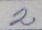
\includegraphics[width=.1\textwidth]{./pics/dos.png} \\
\item alterados con malicia (rayaduras, superposición\ldots{})
\item tachones bienintencionados
\end{enumerate}

\bigskip Sigue \emph{machine learning}
\end{column}
\begin{column}{0.45\columnwidth}
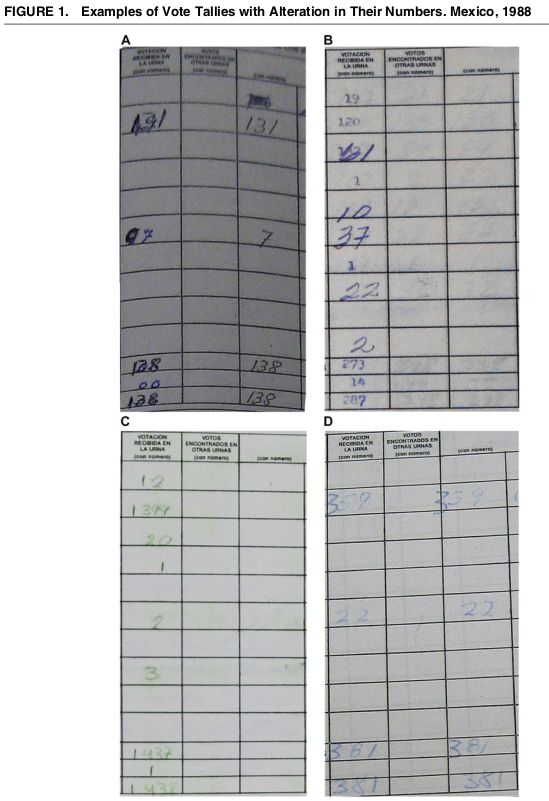
\includegraphics[width=\columnwidth]{./pics/fig1-apsr.png}
\end{column}
\end{columns}
\end{frame}
\begin{frame}[label={sec:org39e51f3}]{Operaron los gobernadores}
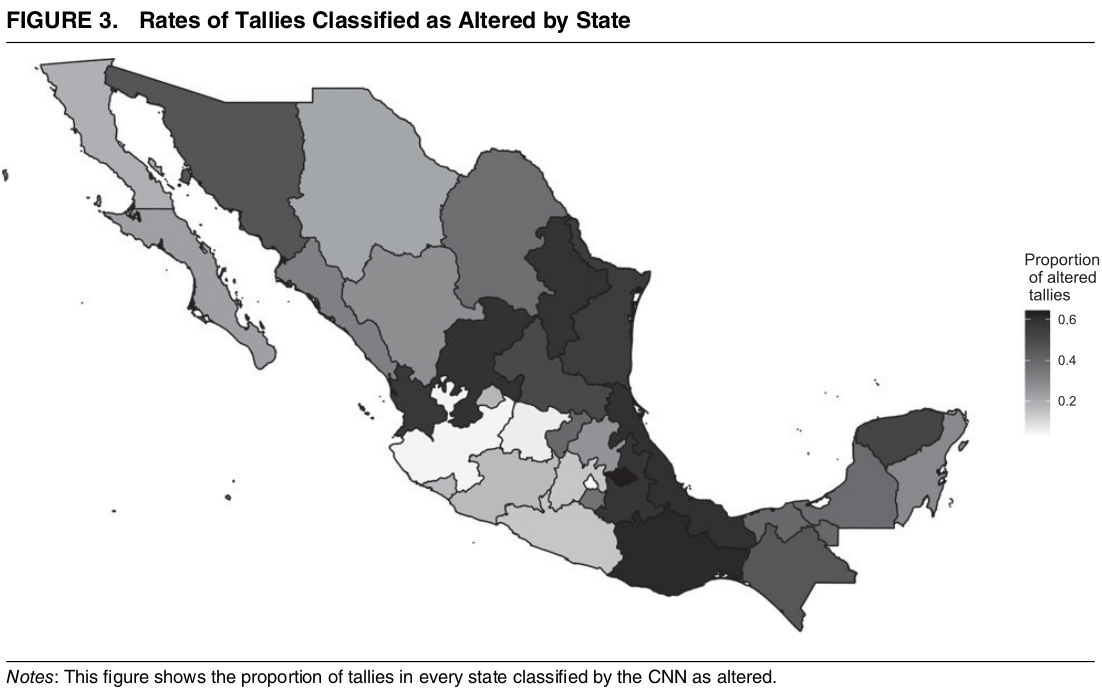
\includegraphics[width=\textwidth]{./pics/mapa-apsr.png} \\
\centering Tasa de error: falso positivo \(\approx 0.07~~~\) falso negativo \(\approx 0.15\)
\end{frame}
\begin{frame}[label={sec:orgac55f49}]{Casillas zapato}
\begin{columns}
\begin{column}{0.5\columnwidth}
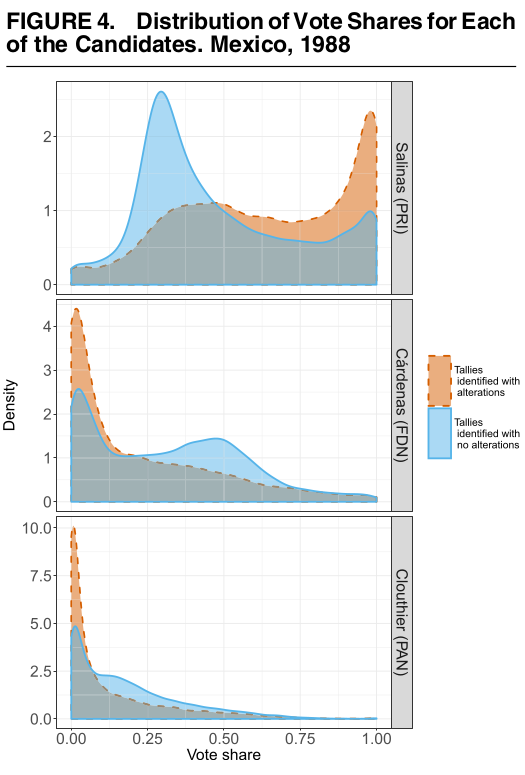
\includegraphics[width=\columnwidth]{./pics/fig4-apsr.png} \\
\end{column}
\begin{column}{0.5\columnwidth}
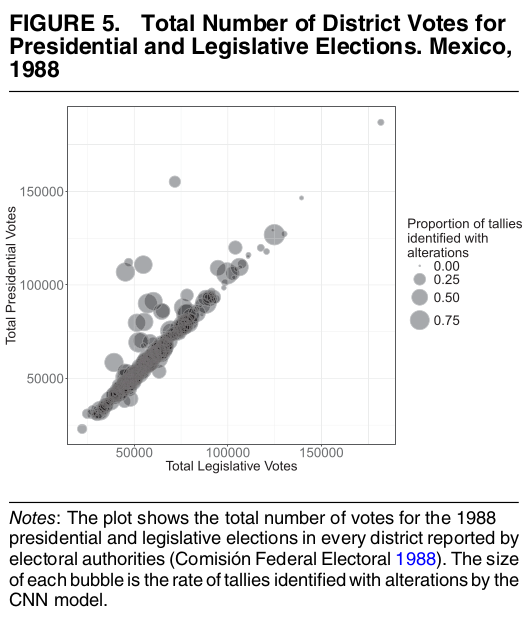
\includegraphics[width=\columnwidth]{./pics/fig5-apsr.png} \\
\end{column}
\end{columns}
\end{frame}
\begin{frame}[label={sec:orgae7a289}]{Correlates}
\begin{tikzpicture}
\node (0,0){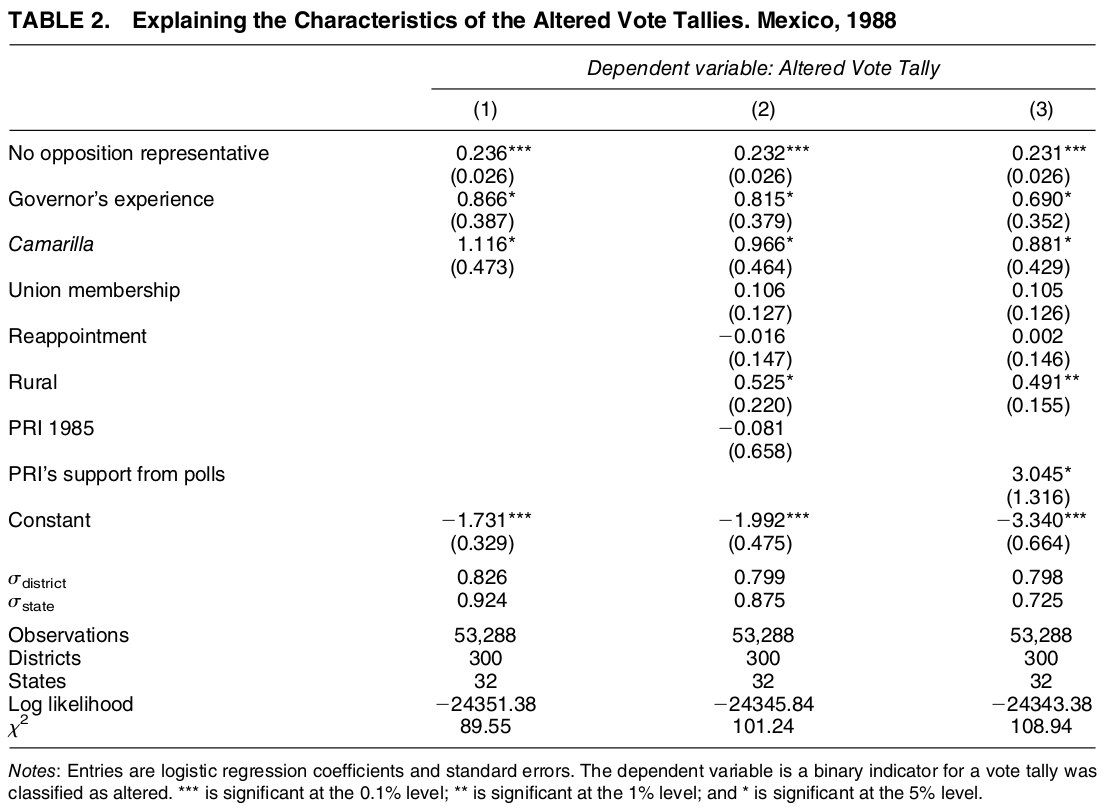
\includegraphics[width=\textwidth]{./pics/reg-apsr.png}};
\fill[draw,fill=none,red,thick] (-1.1,2.6) -- (-0.1,2.6) -- (-0.1,1.1) -- (-1.1,1.1) -- (-1.1,2.6);
\end{tikzpicture}
\end{frame}
\begin{frame}[label={sec:orgaee2438}]{Balance: el estudio sistemático del fraude}
Análisis sistemático confirma

\begin{itemize}
\item \emph{Caída del sistema} no instrumentó un fraude centralizado desde Bucareli
\item sí permitió alterar \(\sim30\%\) actas previo al cómputo distrital, inflando voto Salinas
\item Operación de fuerza bruta por gobernadores "talentosos"
\item ¿CSG se robó la elección o sólo amplió el margen?
\item Obsesión con el \alert{fraude} \newline
1997--2024 quizás matiza
\end{itemize}

\pause \bigskip \centering \alert{¡Gracias Francisco!}
\end{frame}
\end{document}
